\documentclass{standalone}

\usepackage{tikz}
\usepackage{pgfplots}
\begin{document}
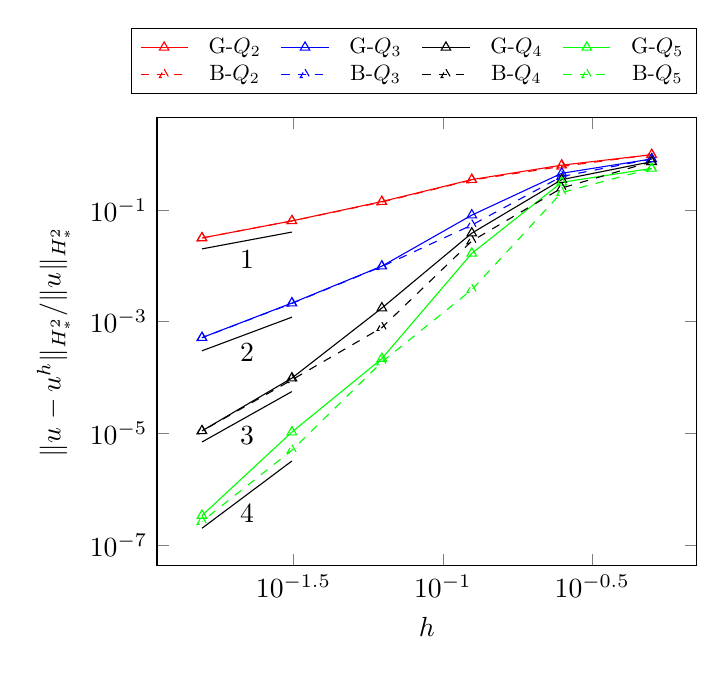
\begin{tikzpicture}
    \begin{loglogaxis}[
        legend columns=4,
    	legend style={at={(1,1.2)}, nodes={scale=0.8, transform shape}, column sep=.2cm},
        xlabel=$h$,
        ylabel=${\|u_{}-u^{h}\|_{H^2_*}}/{\|u_{}\|_{H^2_*}}$ 
    ]


    \addplot [color=red,mark=triangle] plot coordinates {

        (.5,    0.970233)
        (.25,   0.630331)
        (.125,   0.347793)
        (.0625,   0.140633)
        (0.03125,   0.063464)
        (0.015625,   0.0313622)
    };

    \addplot [color=blue,mark=triangle] plot coordinates {

        (.5,    0.812838)
        (.25,   0.451057)
        (.125,   0.0804161)
        (.0625,   0.00981443)
        (0.03125,   0.00214694)
        (0.015625,   0.000516027) 
    };

    \addplot [color=black,mark=triangle] plot coordinates {

        (.5,    0.727478)
        (.25,   0.347299)
        (.125,   0.0382459)
        (.0625,   0.00174571)
        (0.03125,   9.75601e-05)
        (0.015625,  1.10561e-05)
    };

    \addplot [color=green,mark=triangle] plot coordinates {

        (.5,     0.5517)
        (.25,   0.310648)
        (.125,   0.0166288)
        (.0625,   0.000217162)
        (0.03125,   1.05336e-05)
        (0.015625,   3.38835e-07)
    };

    
    \addplot [color=red,mark=triangle, dashed] plot coordinates {

        (.5,    0.970233)
        (.25,   0.598473)
        (.125,   0.341423)
        (.0625,   0.137625)
        (0.03125,  0.0633613)
        (0.015625,  0.0313625)
    };

    \addplot [color=blue,mark=triangle, dashed] plot coordinates {

        (.5,    0.812838)
        (.25,   0.395827)
        (.125,   0.0533701 )
        (.0625,   0.00965695)
        (0.03125,  0.00211437)
        (0.015625,  0.000513982)
    };

    \addplot [color=black,mark=triangle, dashed] plot coordinates {

        (.5,    0.727478)
        (.25,   0.245455)
        (.125,    0.0276997)
        (.0625,    0.000779448)
        (0.03125,  9.08055e-05)
        (0.015625,  1.10167e-05 )
    };

    \addplot [color=green,mark=triangle, dashed] plot coordinates {

        (.5,    0.548646 )
        (.25,   0.204253 )
        (.125,   0.0037194)
        (.0625,   0.000188883)
        (0.03125,  4.98227e-06)
        (0.015625,  2.65114e-07)
    };

    \addplot [black] plot coordinates {

        (0.03125,       0.0400 )
        (0.015625,      .02 )
    } node[pos=0.5,anchor=north]{$1$};

    \addplot [black] plot coordinates {

        (0.03125,       0.0012 )
        (0.015625,      .0003 )
    } node[pos=0.5,anchor=north]{$2$};

    \addplot [black] plot coordinates {

        (0.03125,       5.6000e-05 )
        (0.015625,      7e-6 )
    } node[pos=0.5,anchor=north]{$3$};

    \addplot [black] plot coordinates {

        (0.03125,       3.2000e-06 )
        (0.015625,      2e-7 )
    } node[pos=0.5,anchor=north]{$4$};


    \legend{G-$Q_2$\\G-$Q_3$\\G-$Q_4$\\G-$Q_5$\\B-$Q_2$\\B-$Q_3$\\B-$Q_4$\\B-$Q_5$\\}
    \end{loglogaxis}
\end{tikzpicture}

\end{document}


% 1.08115   0.970233
% 0.792129   0.630331
% 0.322907   0.347793
% 0.0307356   0.140633
% 0.00444968   0.063464
% 0.00106043   0.0313622

% 0.857518   0.812838
% 0.385025   0.451057
% 0.0225406   0.0804161
% 0.00041709   0.00981443
% 1.09308e-05   0.00214694
% 4.26084e-07   0.000516027

% 0.595125   0.727478
% 0.265113   0.347299
% 0.00797683   0.0382459
% 0.000106357   0.00174571
% 7.13069e-07   9.75601e-05
% 6.78607e-09   1.10561e-05

% 0.435502   0.5517
% 0.20598   0.310648
% 0.00330122   0.0166288
% 5.16129e-06   0.000217162
% 1.30976e-07   1.05336e-05
% 8.33014e-10   3.38835e-07